\begin{figure}[h!]
    \centering
    \setlength{\tikzunit}{\textwidth/33}
    \begin{tikzpicture}[scale=1, x=\tikzunit,y=\tikzunit]
        \tikzstyle{every node}=[font=\tiny]
        \node(0,0) {};
        \draw( 0.0, 0.0) node{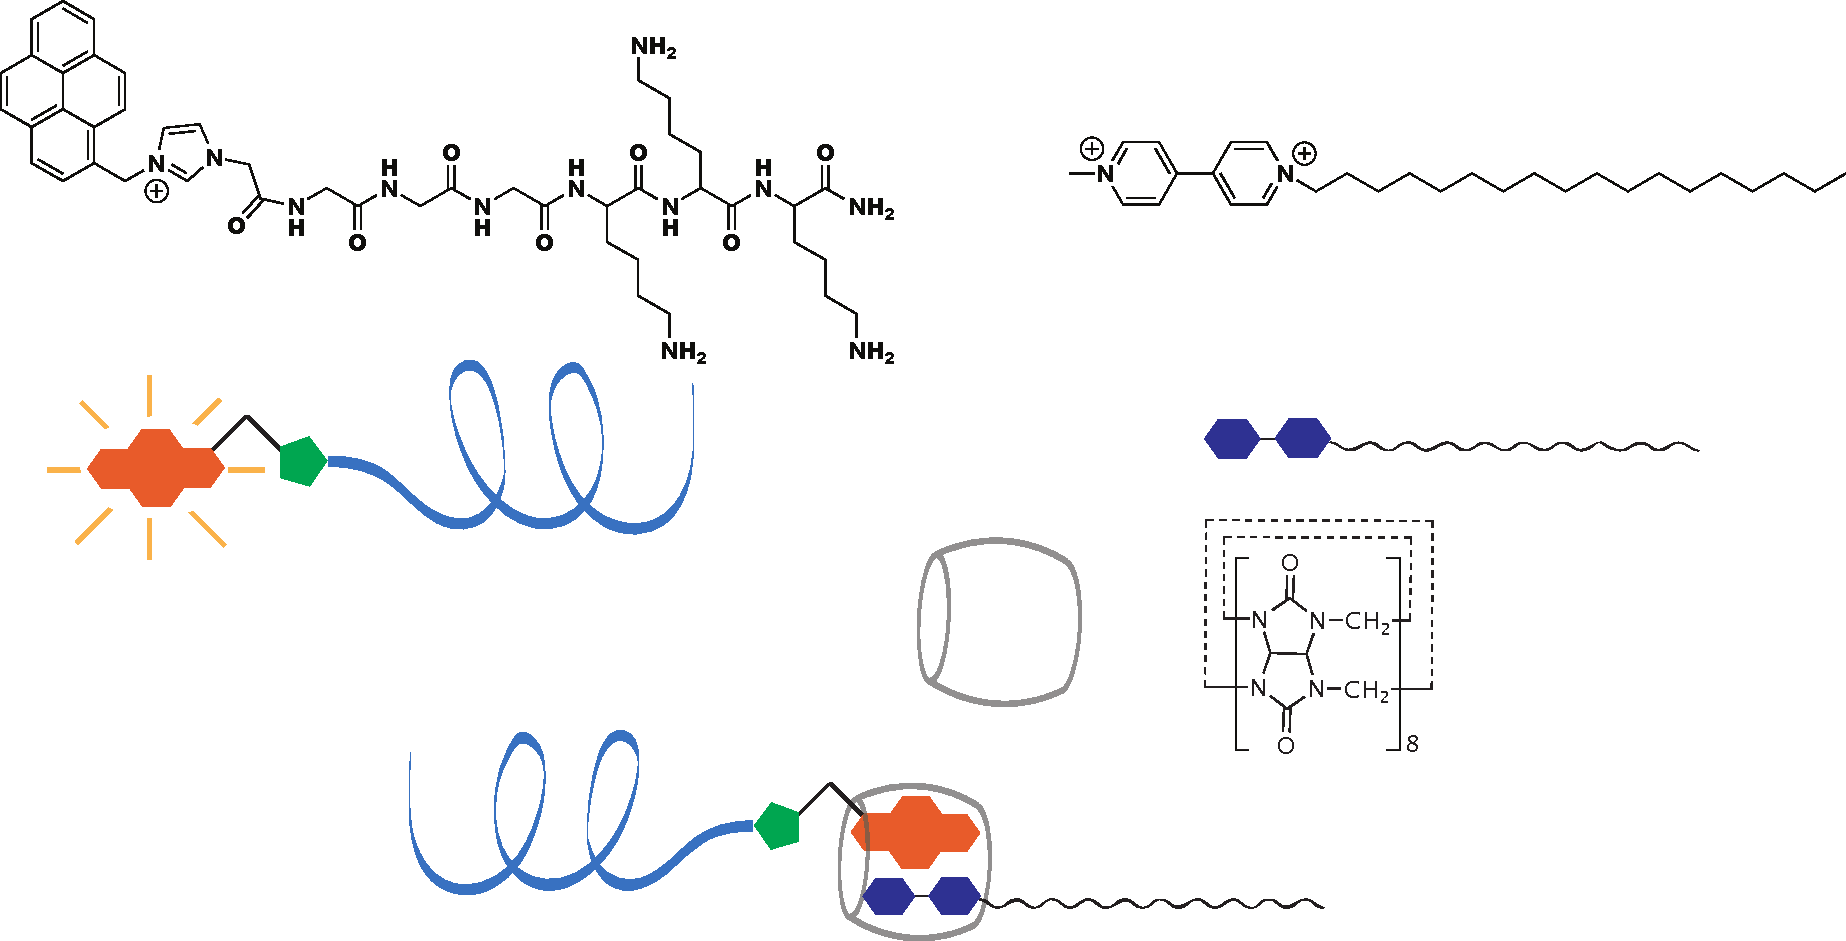
\includegraphics[height=8\tikzunit]{illustration1.pdf}};
%        \draw[step= .5,color=gray,thin,dashed](-8,-4) grid ( 8, 4);
%        \draw[step=1.0,color=gray]            (-8,-4) grid ( 8, 4);
%        \draw[step=4.0,color=black]           (-8,-4) grid ( 8, 4);
        \draw(-4.5, 1.5) node{\ce{PylmGGGKKK} (\textbf{1})};
        \draw(-4.5, 1.00) node[rotate=90]{$\equiv$};
        \draw(-8.25,3.75) node{\textbf{a)}};
        \draw( 4.0, 1.5) node{\ce{MV^{2+}(CH2)17CH3} (\textbf{2})};
        \draw( 4.0, 1.00) node[rotate=90]{$\equiv$};
        \draw( .75, -1.25) node{CB[8]};
        \draw( 1.75, -1.25) node{$\equiv$};
        \draw( -.25, -1.25)  node[left]{\footnotesize Switch of fluoresence};
        \draw( 0.0, -4.25) node{Peptide amphiphile};

        % an arrow
        \path[draw,thick,->] (-0.25,0.25) -- (-.25,-2.25);
    \end{tikzpicture}
    \caption{scientific illustration}
    \label{fig:struct2} 
\end{figure}
